% !TeX spellcheck = uk_UA
\documentclass{article}

\usepackage{graphicx}
\graphicspath{{./images}}
\usepackage{float}
\usepackage{xcolor}
\usepackage{textcmds}
\usepackage{listings}
\definecolor{codegreen}{rgb}{0,0.6,0}
\definecolor{codegray}{rgb}{0.5,0.5,0.5}
\definecolor{codepurple}{rgb}{0.58,0,0.82}
\definecolor{backcolour}{rgb}{0.95,0.95,0.92}

\lstdefinestyle{mystyle}{
	backgroundcolor=\color{backcolour},   
	commentstyle=\color{codegreen},
	keywordstyle=\color{magenta},
	numberstyle=\tiny\color{codegray},
	stringstyle=\color{codepurple},
	basicstyle=\ttfamily\footnotesize,
	breakatwhitespace=false,         
	breaklines=true,                 
	captionpos=b,                    
	keepspaces=true,                 
	numbers=left,                    
	numbersep=5pt,                  
	showspaces=false,                
	showstringspaces=false,
	showtabs=false,                  
	tabsize=2
}

\lstset{style=mystyle}
\usepackage[T1,T2A]{fontenc}
\usepackage[utf8]{inputenc}
\usepackage[english, ukrainian]{babel}
\begin{document}
	\begin{center}
		\textbf{
			\large{
			КИЇВСЬКИЙ НАЦІОНАЛЬНИЙ УНІВЕРСИТЕТ ІМЕНІ ТАРАСА ШЕВЧЕНКА \\
			МЕХАНІКО-МАТЕМАТИЧНИЙ ФАКУЛЬТЕТ \\
		    КАФЕДРА ТЕОРІЇ ЙМОВІРНОСТЕЙ, СТАТИСТИКИ ТА АКТУАРНОЇ МАТЕМАТИКИ \\
			\hfill \break
			ДИПЛОМНА РОБОТА \\
			НА ЗДОБУТТЯ СТУПЕНЯ МАГІСТРА \\
			 НА ТЕМУ: \\
			\hfill \break
			"ПЕРЕНОС СТИЛЮ НА ЗОБРАЖЕННЯХ ЗА ДОПОМОГОЮ ГЕНЕРАТИВНИХ ЗМАГАЛЬНИХ НЕЙРОННИХ МЕРЕЖ" \\
			}	
		}
	\end{center}
	\hfill\break
	\hfill \break
	\hfill \break
	\begin{flushright}
		\textbf{
			Виконав: \\
			студент 2 курсу магістратури \\
			механіко-математичного факультету \\
			спеціальності «Статистика» \\
			Ширченко Максим Вікторович \\
			\hfill \break
			Науковий керівник: \\
			кандидат фізико-математичних наук, \\
			доцент кафедри теорії ймовірностей, \\
			статистики та актуарної математики \\
			Голомозий Віталій Вікторович \\
			\hfill \break
			Допустити до захисту ДЕК \\
			Протокол No \rule{1cm}{0.4pt} від \rule{1cm}{0.4pt} р. \\
			\hfill \break
			Зав. кафедрою \\
			\rule{1.5cm}{0.4pt} Мішура Ю.С.
		}
	\end{flushright}
	\hfill \break
	\hfill \break
	\hfill \break
	\hfill \break
	\begin{center} 
		\textbf{КИЇВ \\ 2021}
	\end{center}
	\thispagestyle{empty}
	\newpage
	
	\tableofcontents
	\newpage
	\section{Вступ}
	\quad На початку 21 століття комп'ютери могли робити безліч складних речей, деколи навіть переважаючи людей. Комп'ютер міг перемогти вас в шахи, допомогти знайти щось корисне, чи навіть допомогти тримати в безпеці ваш будинок. Все це за допомогою машинного навчання (ML,  скорочено від  machine learning). Алгоритми машинного навчання дуже добре справляються з двома задачами - класифікації (присвоєння данним мітки класу) та регресії (передбачення данних). Все це через їх здібність до \qq{запам'ятовування} шаблонів в данних, переданих для навчання. Але данний клас алгоритмів стикається з проблемою, коли потрібно згенерувати якісь данні. З їх допомогою можна передбачити ціни, знайти об'єкти на зображеннях, але будь-яка спроба згенерувати будь-який контент, для прикладу, зображення або ж звук, закінчиться невдачею. Тому потрібне було нове рішення - здатне справитись з такого типу завданнями. \\
	\null\quad В 2014 році Ян Гудфелоу, на той час аспірант Монреальського університету, створив модель генеративних змагальних нейронних мереж (Generative Adversarial Networks; GAN). Ці моделі були не першими в області генерації данних, але суттєво перевершували всі наявні по якості генерації контенту. За допомогою тренування двох нейронних мереж, які конкурують між собою, з'явилась можливість генерувати зображення, якості, не гіршої як у фотографій, перетворювати нарис в повноцінну картину, пейзаж в фотографію і так далі. \\
	
	\begin{figure}[H]
		\centering
		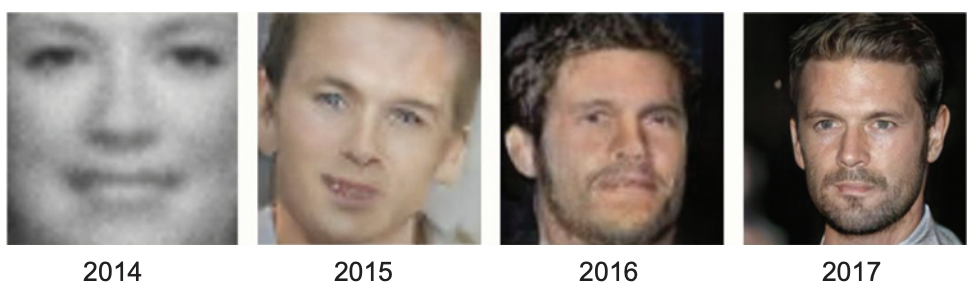
\includegraphics[scale=0.6]{faces.png}
		\caption{Еволюція генерації портретних зображеннь за допомогою GAN}
	\end{figure} 

	\null\quad Ціль данної роботи дослідити процес генерації зображеннь та переносу стилю за допомогою генеративних змагальних нейронних мереж. Для цього потрібно розібрати як архітектуру моделі, так і архітектуру нейронних мереж, які можна використовувати для генерації. Важливо зрозуміти процес навчання цієї моделі, як він проходить і чому це працює. Також в цій роботі я спробую різні моделі, порівняю використання ними ресурсів, швидкість їх навчання та генерації зображеннь. Не менш важливою частиною будуть блоки з аналізом нюансів архітектури, як кожна зміна впливає на генерацію та які може викликати проблеми. Спробуємо різні моделі для переносу стилю на зображення, намагаючись надати нового стилю як всьому зображенню, так і певним його частинам. \\
	\null\quad Актуальність роботи полягає в широкому застосуванні генерованого контенту в нашому житті. Ми кожен день зустрічаємось з ним в соціальних мережах, приміряючи нові фільтри на наші фотографії. Зараз є багато нетривіальних використань генеративних моделей, таких як збільшення роздільної здатності зображення або ж відновлення пошкоджених частин зображення. Використовуючи це ми можемо отримати чіткіше зображення з мікроскопу або телескопу. Приклад зображено на рисунку 2. Вражає, чи не так?
	\begin{figure}[H]
		\centering
		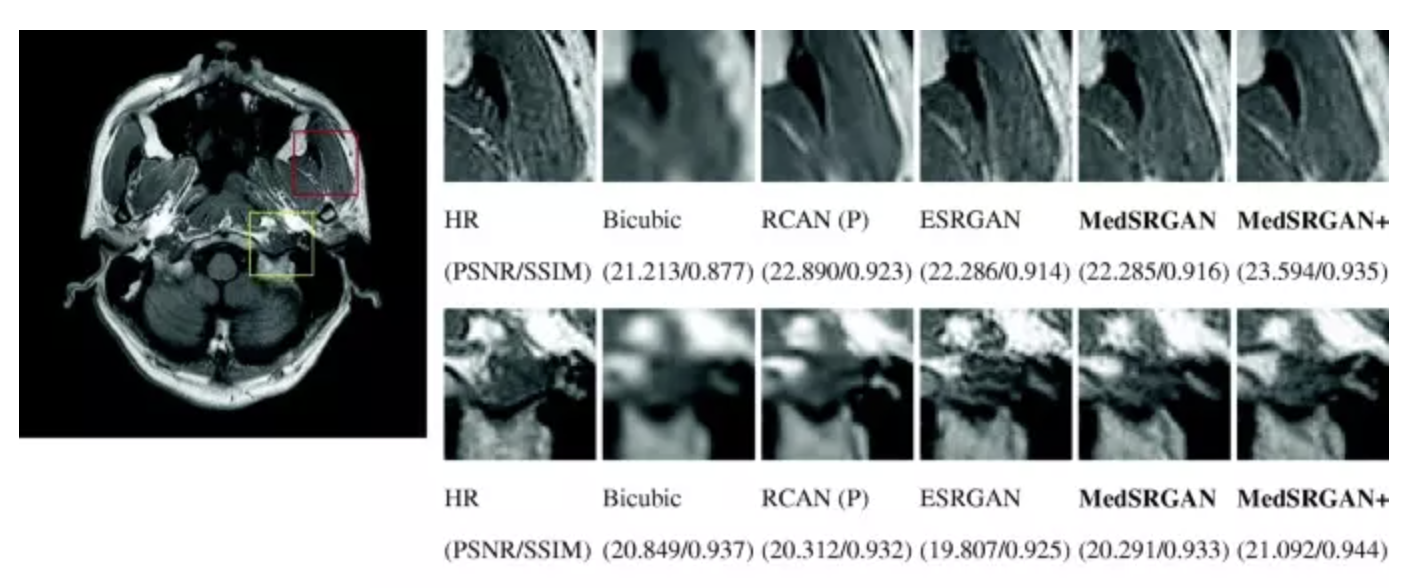
\includegraphics[scale=0.4]{medicine.png}
		\caption{Приклад збільшення роздільної здатності зображення за допомогою GAN в медицині}
	\end{figure} 
	\null\quad Одним із яскравих прикладів використання генеративних моделей є додаток Canvas від немаловідомої компанії Nvidia. Основний його функціонал - перетворення нарису в повноцінний пейзаж. Ви можете додати різні типу об'єктів - гори, поля, озера, вибрати пору року або ж навіть час доби. Результати вражають.
	\begin{figure}[H]
		\centering
		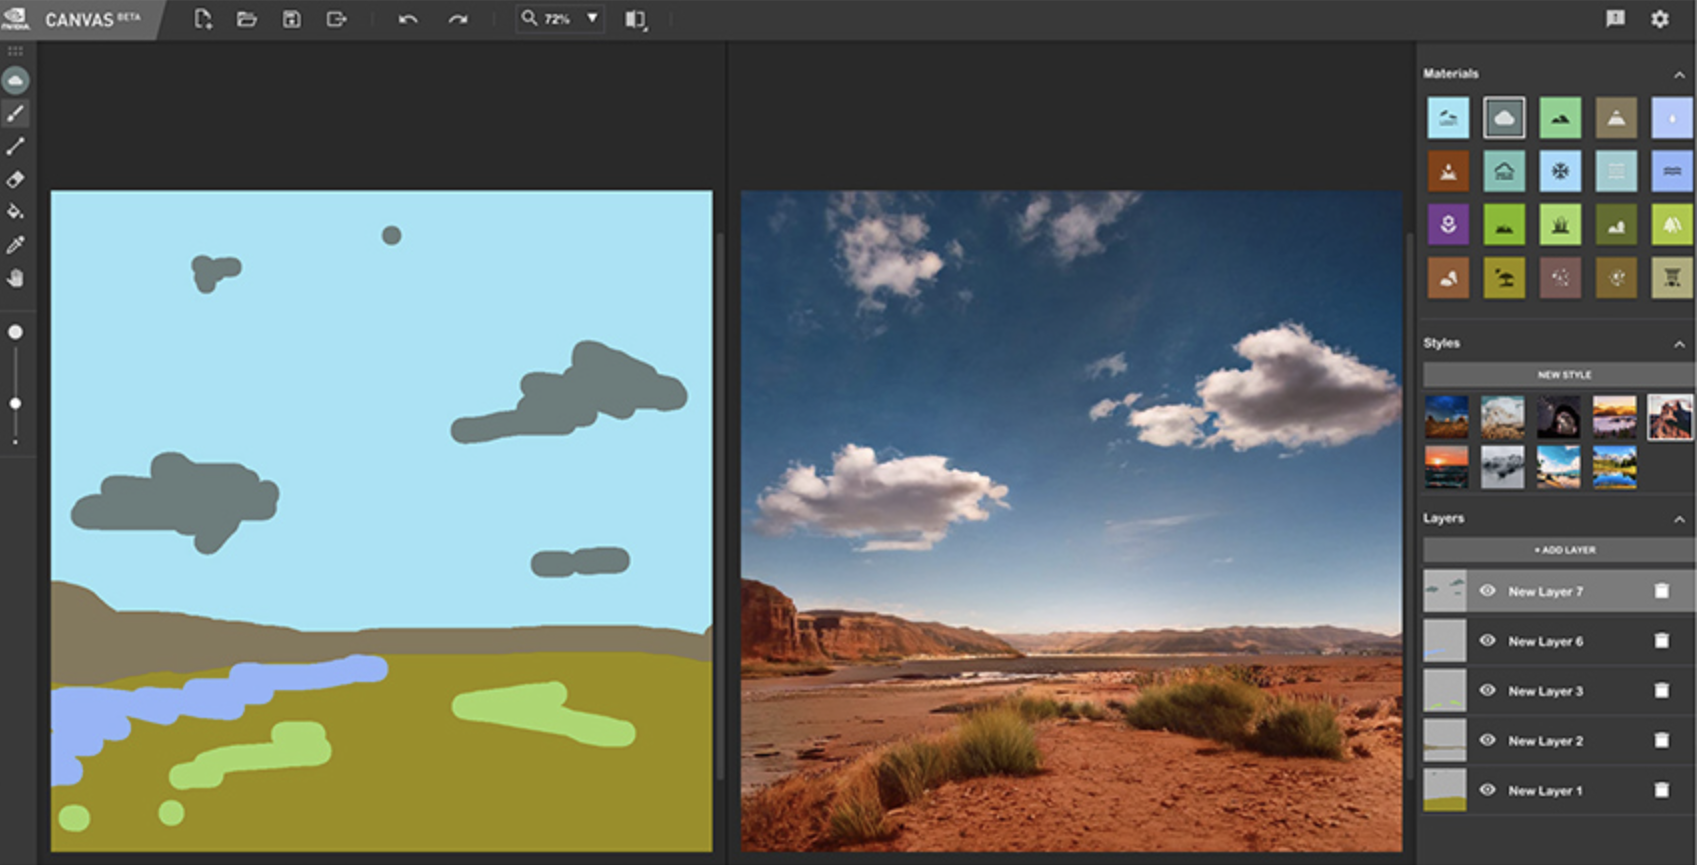
\includegraphics[scale=0.3]{nvidia_canvas.png}
		\caption{Результи роботи додатку Canvas від Nvidia}
	\end{figure} 
	\null\quad Але для досягнення таких результатів потрібно чітко розуміти як працюють генеративні моделі. Є дуже багато вузьких місць в яких потрібно розібратись, що можливо лише при достатніх знаннях теоретичної частини.
	
	\section{Теоретична частина}
	\subsection{Основна ідея моделі}
	\null\quad Генеративні змагальні нейронні мережі - це клас алгоритмів машинного навчання, що працює за допомогою двох нейронних мереж. Завдання першої генерувати контент із випадкового вектору певного розподілу - відповідно називається вона генератор. Завдання іншої відрізняти згенерований контент від реального - далі будемо називати її дискримінатор. \\
	\null\quad Слово \qq{генеративні}  означає основне завдання моделі - генерувати данні. Наважливо чи це звук, картинки, відео чи щось інше. Все що ви передасте в якості набору данних для тренування. \\
	\null\quad Слово \qq{змагальні} описує процес навчання моделі. Під час навчання генератор і дискримінатор намагається конкурувати один з одним - генератор вчиться породжувати контент який би дискримінатор не зміг відрізнити від реального, поданого на вхід для навчання. Дві нейронні мережі постійно змагаються. Для того щоб відрізнити згенерований контент від реального, породженого кращим генератором, покращується дискримінатор і навпаки. \\
	\null\quad І нарешті слово \qq{мережі} позначає клас моделей, які використовуються для генератора та дискримінатора. В залежності від складності моделі мережі можуться варіюватись від простої повнозв'язної мережі до складних згорткових моделей та інших. \\
	\null\quad Як це все працює? Якщо говорити більш технічними термінами, генератор намагається породжувати контент з характеристиками, які він знаходить в контенті, взятому з тренувального наборого данних. Його можна розглянути як класифікатор навиворіт. Класифікатор намагається знайти певні характеристики в наборі данних, тоді як генератор намагається ці характеристики відтворити. \\
	\null\quad Навчання генератора контролюється згідно результів дискримінатора. Якщо дискримінатор хибить і позначає згенерований контент як реальний, тоді модель генератору отримає хороший знак про те що породженні данні дуже схожі на реальні. І навпаки, якщо дискримінатор правильно класифікує всі зображення як згенеровані, генератор отримує відгук про те що данні не схожі на реальні і моделі потрібно покращуватись. \\
	\null\quad Також постійно покращується і дискримінатор. Йому передаються для навчання поміченні данні про реальний і згенерованний контент.  Тому кожен об'єкт, породжений генератором і неправильно класифікований дискримінатором робить другого краще. \\
	\subsection{Постановка задачі генерації зображення}
	\null\quad Одна із основних задач данної роботи є генерація зображень, схожих на зображення, які були подані на вхід моделі.  \\
	\null\quad Більш формально, нехай $X$ - набір зображень (далі будемо позначати зображення літерою $x$), який буде використовуватись для тренування моделі. Якщо ми маємо $n$ зображень і збираємочь генерувати кольорові зображення, кожне розміру $(w, h)$, тоді, враховуючи те, що кожен піксель в зображенні відповідає трьом цифрам - ступеню насиченості червоного, зеленого і синнього кольорів (якщо зображення збережено в кольоровій схемі RGB), $X$ буде тензором розміру $(n, w, h, 3)$. Для генерації чорно-білих зображень розмір тензору X буде $(n, w, h)$, так як кожен піксель буде відповідати тільки одній цифрі -  ступеню насиченості сірого. Далі введемо ймовірнісний простор $\Omega$, та випадкову величину $z: \Omega \rightarrow X$ таку, підмножина X, на якій щільність $p(z)$ ненульова - це певний клас зображень, який ми збираємось генерувати, наприклад фотографії облич. Тому маємо на вхід вибірку випадкових незалежних однаково розподілених величин, зо означають певний клас зображень $\{x_i, i \in [1, N], x_i \sim p(x)\}$. Далі введемо ймовірнісний простір $Z = R^n$ і випадкову величину $z: \Phi \rightarrow Z$, з розподілом ймовірностей, що має щильність $q(z)$. $D: X \rightarrow (0, 1)$ - функція-дискримінатор, вона показує з якою ймовірністю, зображення $x$, взяте з $X$,  відноситься до класу зображень, який ми збиражмось генерувати. $G: Z \rightarrow X$ - функція-генератор, вона приймає $z \in Z$ і повертає як результат об'єкт з простору X, в нашому випадку зображення. Припустимо ми маємо ідеальний дискримінатор, який для кожного $x \in X$  показує вірогідність входження в ${x_i}$.  Нам потрібно навчитись \qq{обманювати} ідеальний дискримінатор, тобто максимізувати вірогідність його відгуку на згенерованих данних. Тобто ідеальний генератор знаходиться як $$G_{ideal} = arg \max_{G} E_{z \sim q(x)} D(G(z))$$\\

	\begin{figure}[H]
		\centering
		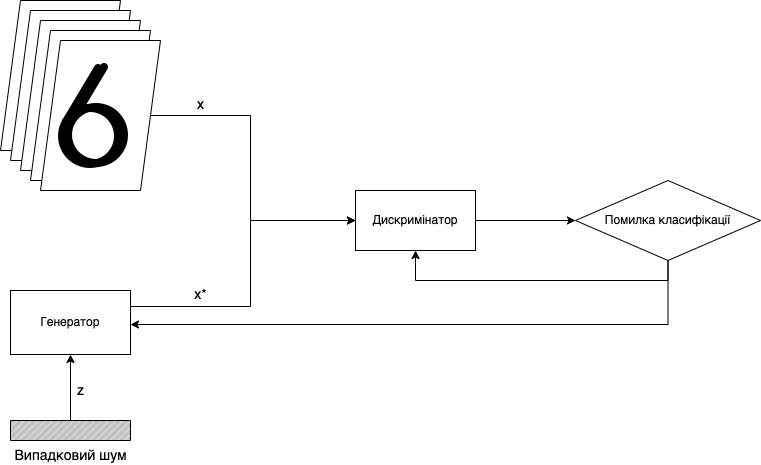
\includegraphics[scale=0.3]{scheme.png}
		\caption{Схема генерації зображення за допомогою GAN}
	\end{figure}
	Під час аналізу різних моделей для виконання цієї задачі ми розглянемо такі питання:
	\begin{enumerate}
		\item Якість генерації зображень.
		\item Час та складність тренування.
		\item Вибір оптимізатора та архітектури.
		\item Використання ресурсів та час генерації зображень.
	\end{enumerate}
  \subsection{Навчання генеративних змагальних мереж}
  \null\quad В попередньому розділі ми вже ввели всі базові поняття, тому продовжимо працювати з ними. В реальному світі ідеального генератору зазвичай знайти майже неможливо. Так як завдання дискримінатора в тому, щоб передавати сигнали для навчання генератора, то ідеального дискримінатора не потрібно, достатньо функції яка чітко розділяє згенеровані об'єкти від об'єктів з навчальної вибірки ${x_i}$. Тобто в термінах машинного навчання, нам потрібно натренувати бінарний класифікатор - модель, яка максимізує ймовірність правильної класифікації для об'єктів з ${x_i}$. Для її тренування маємо нескінченну кількість данних. Вибірка складається з об'єднання скінченної ${x_i}$ та поповнюється кожну ітерацію новими згенерованими об'єктами, при цьому в кожного є мітка, згенерований він чи ні. Опишемо процес тренування дискримінатора \\
  \null\quad  Маємо вибірку $\{(x_i, 0), i \in [1, N], x_i \in X, p(x_i) > 0\} \cup \{(G(z), 0), z \sim q(z)\}$. Визначимо щільність розподілу $f(\xi | \eta = 1) = D(\xi), f(\xi | \eta = 0) = 1 - D(\xi)$. Так як $f(\xi | \eta)$ - переформулювання дискримінатора, який видає ймовірність справжнього об'єкту в вигляді розподілу ймовірностей на інтервалі  $(0, 1)$. Так $D(\xi) \in (0, 1)$, тоді визначення задає щільність розподілу. З цього випливає, що оптимальний дискримінатор можна знайти, як
  $$D^* = f^*(\xi | \eta) = arg \max_{f}f(\xi_1, ... | \eta_1, ...) = arg \max_{f} \prod_{i} f(\xi_i | \eta_i)$$
  Згрупувавши множники для $\eta_i = 0$ і $\eta_i = 1$, маємо:
  $$D^* = f^*(\xi | \eta) = arg \max_{f} \prod_{i} f(\xi_i | \eta_i = 1) \prod_{i} f(\xi_i | \eta_i = 0) = $$
  $$ arg \max_D \prod_{x_i \sim p(x)} D(x_i) \prod_{z_i \sim q(z)} D(G(z_i)) = $$
  $$arg\max_D \sum_{x_i \sim p(x)} log D(x_i) + \sum_{z_i \sim q(x)} D(G(z_i))$$
  І якщо спрямувати розмір вибірки до нескінченності:
  $$D^* = arg \max_D E_{x_i \sim p(x)} log D(x_i) + E_{z_i \sim q(z)} log D(G(z_i))$$
   Тоді маємо наступний ітераційний процес:
   \begin{enumerate}
   	\item Встановлюємо випадковий початковий  $G_0{z}$.
   	\item Починається k-та ітерація , $k = 1...K$
    \item Шукаємо оптимальний для наявного генератора дискримінатор.
    $$D_k = arg \max_D E_{x_i \sim p(x)} log D(x_i) + E_{z_i \sim q(z)} log D(G_{k-1}(z_i))$$
    \item Покращуємо генератор, використовуючи оптимальний дискримінатор.
    $$ G_k = arg \max_D E_{z_i \sim q(x)} D_k(G(z)) $$
    \item  Задача навчання генератора вважається вирішеною, коли $D(x) = 1/2$, для кожного $x$. 
   \end{enumerate}
	\null\quad В оригінальній статті (Ian J. Goodfellow, Jean Pouget-Abadie, Mehdi Mirza, Bing Xu, David Warde-Farley, Sherjil Ozair, Aaron Courville, Yoshua Bengio -  Generative Adversarial Networks)  весь алгоритм складається в одну формулу, що задає мінімакс-гру між генератором і дискримінатором:
	$$\min_G\max_D L(D, G) = E_{ \sim p(x)} log D(x) + E_{z \sim q(z)} D(G(z))$$ 
	\null\quad Як $D$, так і $G$ можуть будуть представленні нейронними мередами, тому всі оптимізації зводяться до алгоритму зворотнього розповсюдження помилки та стохастичного градієнтного спуску. Також нейронна мережа є універсальним оптимізатором, тому не потрібно витрачати час на вибір розподілу $q(z)$. Може бути використаний будь-який в розумних рамках, наприклад нормальний $N(0, 1)$, або рівномірний на інтервалі $[-1, 1]$.\\
	\null\quad Декілька слів про вирішення задачі навчання.  Як згадувалось раніше формула для навчання задає мінімакс-гру між генератором і дискримінатором. Коли одна модель стає кращою, інша стає гіршою.  В цьому налаштуванні можна побачити гру нульової суми, термін з теорії ігор, в якому описується змагання в якому виграш одного з гравців дорівнює суми програшів інших. Кожна така гра має точку рівноваги Неша - така сукупність стратегій та виграшів, при якій жоден із учасників не може збільшити виграш, змінивши вибір стратегії в односторонньому порядку, коли інші учасники не змінюють свого вибору. Названа іменем відомого американського математика та економіста, спеціаліста в галузі теорії ігор, лауреата Нобелівської премії з економіки Джона Форбса Неша, який запропонував цей термін і зробив вагомий внесок у розробку формалізованого опису конфліктних ситуацій, зокрема у визначення формули рівноваги. Для генеративниї нейронних мереж ця рівновага досягається при виконання двох умов:
	\begin{enumerate}
		\item Генератор породжує об'єкти, які не можна відрізнити від реальних об'єктів.
		\item Дискримінатор випадково дає мітки реальним данним (1/2 вірогідність того, що об'єкт реальний)
	\end{enumerate} 
	\null\quad На практиці знайти точно рівноваги для генеративних змагальних мереж майже нереально, через великі трудності з досягненням конвергенції для неопуклих ігор. Взагалі, питання конвергенції для GAN залишається відкритим для дослідження.
	
\end{document}